\documentclass[pageno]{jpaper}

\usepackage[normalem]{ulem}
\usepackage{graphicx}

\newcommand{\name}{Cymric }
\newcommand{\namens}{Cymric}

\begin{document}

\title{\namens: Toward Flexible Exploration of Processor-Near-Memory Architectures}

\date{}
\maketitle

%\thispagestyle{empty}

% Citations to find:
%  Data movement is an increasing source of energy overhead in HPC
%  Micron HMC Announcement
%  Other simulation infrastructures?
%  Assertion: Processor-in-memory was killed by DRAM process
%  Announcement: Micron HMC FPGA board
%  Assertion: GPGPU applications (often) saturate memory bandwidth
%  Assertion: FPGA applications (often) saturate memory bandwidth

\begin{abstract}

This paper reports on the status of {\name}-- an integrated compute-memory system architecture for massively parallel, irregular, data intensive applications.
The major components are a customizable bulk synchronous data parallel architecture integrated with a stacked DRAM memory system and interconnected with a flexible network and package model.
Given the nascent state of processor-near-memory (PNM) architectures, \name has adopted an approach based on the ability to rapidly develop and analyze a space of potential architectural solutions.
The proposed environment is novel in the ability to integrate application binaries, cycle level timing models, and physical models (power, thermal) into a single simulation model.
In particular, we focus on heterogeneous near-memory architectures employing multi-layer (stacked) DRAM technologies with in-stack or in-package multithreaded, data-parallel processing elements running both traditional and irregular CUDA and OpenCL workloads.
The environment couples a customizable \texttt{C++}-based data parallel architecture synthesis/generation framework with microarchitecture level full system simulation models.
We report on the current status, capabilities and future plans. 

%At the start any systematic study of a class of techniques in computer architecture, it is important to specify, broadly, a set of architectures your group intends to explore, a set of applications with which these architectures will be evaluated, a programming model for these applications, and a set of simulation tools to be used to perform these evaluations.
%Collectively, these four traits define a  position on approaching a research topic.
%The authors are focusing on heterogeneous near-memory architectures employing multi-layer (stacked) DRAM technologies with in-stack or in-package multithreaded, data-parallel processing elements running both traditional and irregular CUDA and OpenCL workloads.
%These architectures are being evaluated using a two-pronged approach: (1) a simulation stack composed of the MacSim trace-driven processor and GPU simulator, the Structural Simulation Toolkit (SST) simulation framework, and the CHDL low-level hardware design environment and (2) a CHDL-based FPGA prototyping toolchain.
\end{abstract}

\section{Introduction}
% - Row-buffers are big and allow unrestricted access to memory
% - DDR bandwidths are getting faster at the cost of power
% - Data movement is expensive, period
% - Locating computing closer to memory provides equivalent or better bandwidth
%    - With less energy overhead
%    - With less transfer latency
% - Earlier research into processor-in-memory was hindered by unsuitability of
%   DRAM processes for logic.
% - 3D stacking and novel packaging has renewed interest in PNM.
% - Multithreaded data parallel processors (like GPGPUs) make sense near RAM
%   because of their applications' ability to saturate DRAM bandwidth and re-
%   configurable logic (like FPGAs) makes sense near RAM because of their
%   applications' " " " " bandwidth.
%     - ``But wait!'' you say. Bandwidth is fine. Latency is the name of the
%       game for near-memory.
%       - It's all about the joules.
% - We need simulators to evaluate these processors.

Data movement is responsible for a large portion of the power budget of modern supercomputers.
Techniques for mitigating this cost have focused on reducing the amount, frequency, and cost of long-distance communication, but this still does not address the basic problem of access to data in DRAM.
For memory-intense applications with certain access patterns, the DRAM bandwidth is readily saturated.

A historical approach to solving this problem was PIM, processor-in-memory; placing compute logic on the same die as DRAM.
This provides unhindered access to the entire row buffer, enabling unprecedented bandwidth between the on-memory processing elements and the RAM.
This technique ultimately proved unfeasible in cost-oriented commodity DRAM processes.
They were simply unable to provide fast enough MOSFETs to justify moving any amount of processing into the DRAM.
This frustrating state of affairs received a perturbation when manufacturers began demonstrating successful 3D stacked memory products.
These allow processors to be implemented in suitable processes and stacked under DRAM layers, either directly with through-silicon vias or in the same package.

When a disruptive technology such as 3D-stacked RAM appears, computer architects race to incorporate it into new architectures and characterize them.
The near-memory processing enabled by these stacked RAMs is no different.
This paper describes the set of architectures our group is exploring and the set of tools we are using to evaluate them.

This document is structured as follows:
First we will describe the sets of architectures employing near-memory processing that we are exploring, the programming models exported by these machines, and the benchmark applications we intend to evaluate on them.
In the second section, we will describe the evaluation and prototyping environment we are using to explore these architectures.
We will conclude a quick look at planned future work.


\section{Architectures}
\begin{figure}
  \centering
  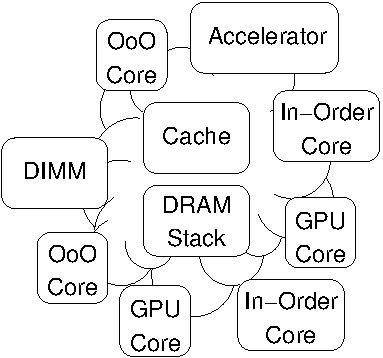
\includegraphics[width=2in]{fig/arch}
  \caption{Thanks to the flexibility of the simulation infrastructure, the system architecture of \name can remain defined only as a set of components. Where these should located and in what topology they should be connected is the topic of future research.}
  \label{fig:arch}
\end{figure}

Figure~\ref{fig:arch} illustrates the architecture of a \name system; notable for its lack of structure.
It is not yet clear at this early point in the development of PNM architectures exactly what their high-level structure should be.
With a flexible simulation infrastructure we will be able to explore a variety of possible system-level architectures, including combinations of:
\begin{itemize}
  \item Networks-on-chip.
  \item In-package integration with DRAM stacks.
  \item 3D-stacked integration with DRAM stacks.
\end{itemize}

Micron's Hybrid Memory Cube (HMC) \cite{hmc} is one of the most promising emerging stacked DRAM technologies.
FPGA products with HMC interfaces have recently been announced. \cite{hmcfpga}
This combination of FPGA and stacked memory is an attractive target for prototype near-memory architectures.
Prototypes built in such a manner would hardly qualify as having PNM architectures, but their designs would share much more with PNM architectures than they would with DDR-based systems.


\section{Evaluation Infrastructure}
The Structural Simulation Toolkit \cite{sst} is central to our evaluation methodology.
SST provides a distributed simulation framework with a versatile, configurable memory system model, including VaultSim, a model of 3D stacked DRAM.
To SST we couple MacSim \cite{macsim}, a trace-driven processor and GPU simulator, and CHDL, a \texttt{C++} hardware design and simulation library.

\begin{figure*}[h!]
  \centering
  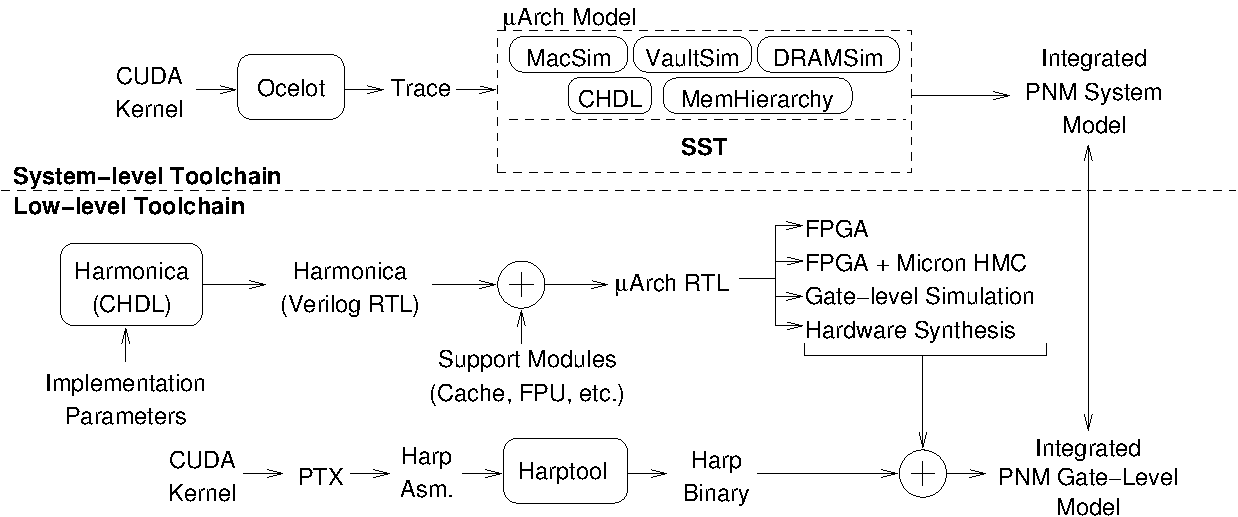
\includegraphics[width=6in]{fig/toolchain}
  \caption{The authors' software infrastructure consists of an RTL CPU design with an enabling hardware design library, a high-level simulation flow, and a low-level implementation flow capable of targeting FPGAs.}
  \label{fig:toolchain}
\end{figure*}


\subsection{MacSim}
MacSim \cite{macsim} is a trace-driven and cycle-level heterogeneous architecture simulator.
It models architectural behaviors such as detailed pipeline stages, multi-threading, and memory systems. 

Micron's Hybrid Memory Cube (HMC) \cite{hmc} is one of the most promising emerging technologies supporting the implementation of near memory architectures.

We can easily explore many points in our architectural design space including ones that exploit HMC as a near memory dram cache alongside an off-chip memory by varying MacSim and VaultSim configurations and assembling different memory hierarchies in the SST configuration.

We can configure MacSim and VaultSim on top of the SST framework so that it models architectures that are of interest.
For example we can form a variety of topologies of VaultSims to get an idea of how different characteristics of HMC as opposed to current DDR-based memory can affect overall system performance when they are employed in different formation.
Specifically we can organize more than one VaultSims so that one of them directly talks to MacSim (Host CPUs or GPUs) while others talk to each other.

Besides, we can vary the number of GPUs, the number of VaultSims, typical DRAM parameters, TSV width, link bandwidth, transaction size, etc to evaluate the sensitivity to parameters in different configurations so that we can get an idea how each and every parameter influences on performance as well as which is the optimal configuration and topology pair before diving into deep exploration.

%We select 29 benchmarks from spec2006 benchmark suite to cover a wide range of application domains. For each benchmark, we use the default input included in its corresponding benchmark suite.


\subsection{HARP and CHDL}
\begin{figure}[h!]
  \centering
  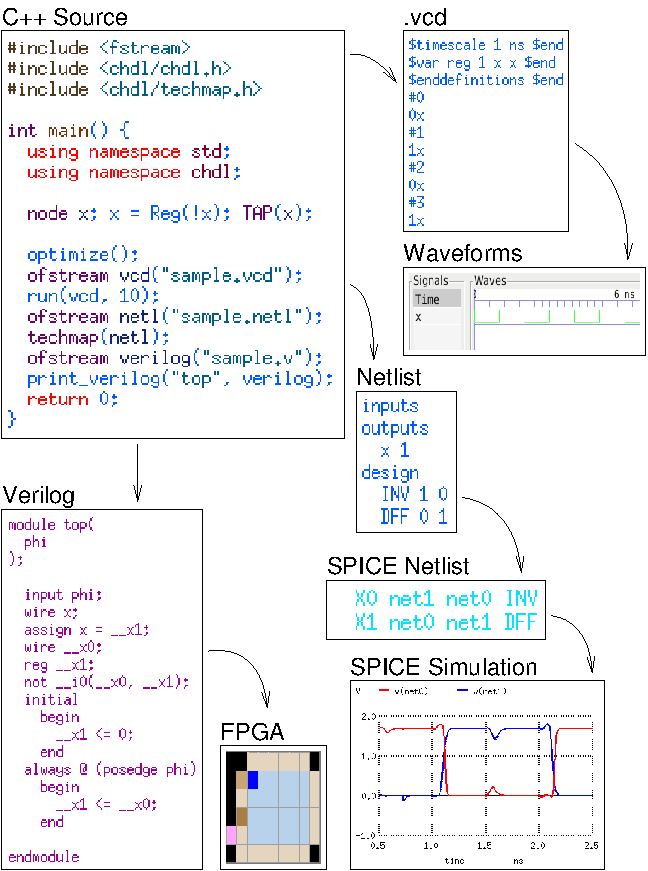
\includegraphics[width=3.5in]{fig/chdl}
  \caption{CHDL is a versatile \texttt{C++} hardware design library supporting a wide range of output formats.}
  \label{fig:chdl}
\end{figure}

An open source \texttt{C++}-based hardware design library called CHDL \cite{chdl} forms the core of the prototyping and gate-level simulation efforts.
CHDL designs are created by writing a high-level description in \texttt{C++}.
These descriptions can be incorporated into a program which, when compiled and run, produces any of a variety of outputs, which can include
\begin{itemize}
  \item Value Change Dump (\texttt{.vcd}) files representing simulation output.
  \item Optimized synthesizable Verilog source code.
  \item Intermediate netlists suitable for circuit-level simulation or place and route.
\end{itemize}
A very brief CHDL example is shown in Figure~\ref{fig:chdl} along with a variety of output formats.

Our ongoing effort to produce a heterogeneous architecture research prototype (HARP) has succeeded in producing a set of instruction set architectures collectively known as the HARP ISA, an assembler/linker/emulator tool, and a parameterized in-order, single-issue, register transfer level implementation called Harmonica.
The HARP ISA is parameterized fully predicated SIMD instruction set intended to be used in a wide range of processor designs.
Because of the parameterized nature of the HARP ISA and the Harmonica implementation thereof, it is versatile, being able to fill multiple roles in the so-called compute hierarchy.

Harmonica is a pipelined processor that issues instructions in-order and allows them to complete out-of-order.
It is built in a modular fashion so that functional units implementing various sets of instructions can be added or omitted as desired.
The minimum pipeline depth is four, but depending on the number of functional units installed and the number of outstanding instructions each might have, the total instructions in flight can be much higher.
Table~\ref{table:harp} provides an example of the range of core sizes and parameters possible with Harmonica.
These are on the small side, lacking floating point units and having relatively small register files.
In the figure, ``gates'' is the total post-optimization number of nand gates, D flip-flops, and inverters in the design.

\begin{table}
  \centering
  \begin{tabular}{ccc|cc}
    Bits&Regs&Lanes&  Gates& Crit. Path (Gates)\\
    \hline
    32  &   8&    1&  31811&           99\\
    32  &  16&    1&  36459&           99\\
    32  &  16&    2&  62295&           99\\
    32  &  16&    8& 217358&           99\\
    32  &  16&   16& 424117&           99\\
    64  &  16&    8& 544835&          105\\
    32  &  16&   32& 864220&           99\\
  \end{tabular}
  \caption{Harmonica implementation of HARP ISA with various parameters. All of these numbers represent integer-only cores with gshare branch prediction.}
  \label{table:harp}
\end{table}

This work does not exist in isolation from the higher-level simulation work.
Using a set of generic interface functions, a CHDL processor model has been demonstrated running within SST, using SST's MemHierarchy interface as its only memory system.
This integration will allow a seamless transition between high-level trace-driven models and low-level synthesizable hardware models and has the added advantage, since SST is a distributed simulation framework, of allowing multiple CHDL processor implementations to be simulated within SST in parallel.

The eventual goal of the HARP project is to run unmodified GPU kernels generated from the PTX intermediate form as well as non-SIMD benchmarks compiled from C.
For now, all of the applications are kernel benchmarks written directly in HARP assembly language.


\subsection{FPGA prototype}
\begin{table}
  \centering
  \begin{tabular}{|l|c|}
    \hline
    \multicolumn{2}{|c|}{Harmonica Core} \\
    \hline
    FPGA:&Stratix III; 113,600 LEs\\
    Operating Freq:&\~90 MHz\\
    RAM(data), ROM(inst):& 1024KB, 1024KB\\
    Regs:& 8 32-bit Regs\\
    %Lanes -> 1
    FPGA Utilization:&4\%  (3,661 / 113,600 ALUTs)\\ \hline \hline
    \multicolumn{2}{|c|}{Full system} \\
    \hline
%FPGA:&Stratix III; 113,600 LEs\\
Operating Freq:&\~62.5 MHz\\
L1 / L2 cache:& 16KB / 128KB\\
Combinational ALUTs:&13\%	(14,446 / 113,600 ALUTs)\\
Total block memory bits:&27\%	(1,505,792 / 5,630,976 )\\
    \hline
%Logic utilization:&	21 %\\
%Regs:& 8 32-bit Regs\\
%No FPu
  \end{tabular}
  \caption{The Harmonica core in its default configuration takes up very little FPGA real estate.}
  \label{table:fpga}
\end{table}

One of the goals of the evaluation toolchain is to have the ability to quickly prototype some subset of the systems we are exploring on an FPGA.
The tools we have developed and adopted allow us to quickly tune system parameters and implement prototypes on FPGA boards and measure their performance.
We can use this process to guide parameter selection in other aspects of architecture simulation.

Our first FPGA board prototype is built around the Harmonica core.
Synthesizable Verilog code for the core was generated by compiling the Harmonica source with GCC and linking against the CHDL library.
This code was then compiled for an Altera Stratix III FPGA using Altera's Quartus II tool suite.
Simple test applications written in HARP assembly like array sum, sieve of Eratosthenes and bubble sort were used to verify the design.
The logic consumption of this simple design was tiny as can be seen in Table~\ref{table:fpga}.
With this flexible toolchain and a customizable ISA and core we are now able to quickly iterate, rapidly implementing modifications to our instruction set, core, and system architecture.
For example, adding support for new instructions, new types of branch predictor, different floating point unit designs, new cache designs and memory controllers, etc. was relatively easy.

Once the Harmonica core was running on the FPGA we integrated it with more complex modules to create a more complete system.
A 2-level non-blocking write-back cache written in Verilog was created and interfaced with the CHDL-based Harmonica code.
This cache is also parameterized.
Its size and number of ways, can be changed, and it can be used in multi-level configurations.
After integrating the cache we began integrating a DDR2 memory controller generated with Altera's MegaWizard tool with the core and cache.
The logic consumption of this design can be seen in Table~\ref{table:fpga}.

In summary, we created a system-level prototype consisting of a highly configurable core, cache and DDR2 memory controller.
Each of these components was individually tested before integration.
This flow will be helpful for future work in which we plan to use it to explore PNM architectures, e.g. by interfacing the FPGA prototype with Micron's Hybrid Memory Cube.
We will only have to obtain a new memory controller IP either from the vendor or add changes to an existing one.
This will also us to do various studies like what configuration of the logic layer will be best suited for this type of memory architecture and examine critical paths.


\section{Future Work}
The work remaining is non-trivial and includes:

\begin{itemize}
  \item Evaluate system architectures and establish a baseline
  \item Expanding the feature set of Harmonica
  \item Performance optimization for both FPGA and silicon targets
  \item Building a capable PTX to HARP Translator
  \item Implementing a custom memory controller
  \item Adding support for HMC to the cache model
\end{itemize}


\section{Related Work}
%..

PIM systems have been researched intermittently for a long time now. Most of the work involved major modifications to the DRAM architecture and they used simulators to shows the benefit. Many designs also used SRAM for the near memory \cite{diva}. Among the initial works, one version developed by \cite{terasys} built PIM as a SIMD array of ALUs next to an SRAM.
%[uiuc] uses execution driven simulators to design a co-processor system with the co-processor having scratch pad memory.
\cite{diva} was a popular PIM based architecture where they simulated using RSIM and also created a first prototype. The fabricated prototype ASIC showed encouraging results but again it is time consuming to redesign prototypes for new architecture. It also requires a significant change to DRAM architecture.
We did not find much literature which talked about providing enough flexibility to explore different architectures of not just the PIM node but of the overall system. They were either more focused on creating prototypes based on a fixed architecture \cite{diva}\cite{flexram}\cite{iram} or its advantage for certain types of applications at a high level using simulations \cite{multimedia_fpga}\cite{sram_based_simulation}\cite{blast}.

%the downside being it required its own highly programming language with no room for flexibility and given availability of FPGAs we already have this kind of implementation.

%[DIVA] M. Hall, P. Kogge, J. Koller, P. Diniz, J. Chame, J. Draper, J. LaCoss, J. Granacki, A. Srivastava, W. Athas, J. Brockman, V. Freeh, J. Park, and J. Shin. Mapping Irregular Applications to DIVA, A PIM-based Data-intensive Architecture. In Proceedings of the Supercomputing 1999, 1999
%[FlexRam] Y. Kang, M. Huang, S. Yoo, Z. Ge, D. Keen, V. Lam, P. Pattnaik, and J. Torrellas. FlexRAM: Toward an Advanced Intelligent Memory System. In International Conference on Computer Design (ICCD), 1999.
%[IRAM] D. Patterson, T. Anderson, N. Cardwell, R. Fromm, K. Keeton, C. Kozyrakis, R. Thomas, and K. Yelick. A Case for Intelligent RAM. IEEE Micro, 17(2):3444, 1997
%[Blast]An Efficient PIM (Processor-In-Memory) Architecture for BLAST Jung-Yup Kang, Sandeep Gupta,Jean-Luc Gaudiot
%[uiuc] MingliangWei, Marc Snir, Josep Torrellas and R. Brett Tremaine. A Near-Memory Processor for Vector, Streaming and Bit Manipulation Workloads 
%[terasys_1995]Gokhale, M. et al., "Processing in memory: the Terasys massively parallel PIM array"
%[ActivePages] M. Oskin et al., Active Pages: A computation model for intelligent memory, IEEE, 1999.
%[multimedia_fpga] Marco Lanuzzaet al., "Cost-Effective Low-Power Processor-In-Memory-based Reconfigurable Datapath for Multimedia Applications"
%[sram_based_simulation] N.Venkateswaran et al., "Memory In Processor: A Novel Design Paradigm for Supercomputing Architectures"


\bstctlcite{bstctl:etal, bstctl:nodash, bstctl:simpurl}
\bibliographystyle{IEEEtranS}
\bibliography{references}

\end{document}

